\chapter{Reconstruction de la masse des bosons W et Z dans l'ILD}
\label{chap.ild}
Nous allons, dans ce chapitre, étudier les performances du Grand Détecteur International, introduit dans le chapitre~\ref{chap.ilc}, avec le concept de calorimètre à lecture semi-digitale. Nous rappellerons, dans un premier temps, les performances requises par le système de calorimètres de l'ILD. Puis, nous présenterons la méthode de suivi de particules utilisée dans l'ILD. Nous étudierons ensuite les performances de l'ILD avec le SDHCAL pour la reconstruction de l'énergie des jets et pour l'identification des bosons W et Z lorsqu'ils se désintègrent en paire de quark ou d'anti-quark ou en paire quark-antiquark. 
\minitoc
\newpage

%%%%%%%%%%%%%%%%%%%%%%%%%%%%%%%%%%%%%%%%%%%%%%%

\section{Introduction}
\label{sec.jetintro}
Dans le chapitre~\ref{chap.ilc}, nous avons décrit le programme de physique du Collisionneur Linéaire International. De nombreux états finals intéressants comportent les bosons W et Z. Ces deux bosons ont des masses très proches ($m_W=80.385\pm0.015~GeV$ et $m_Z=91.176\pm0.0021~GeV$). C'est pourquoi une identification efficace et une bonne séparation de ces bosons sera nécessaire. De plus, ces deux bosons se désintègrent majoritairement en hadrons (67.6$\%$ pour le W et 69.9$\%$ pour le Z), ce qui entraîne le développement de jets. Ainsi, la résolution en énergie des jets, souvent notée $\alpha/\sqrt{E}$, sera un facteur très important pour les détecteurs de l'ILC. Une étude préliminaire \cite{brient} montre qu'une résolution en énergie des jets de $30\%/\sqrt{E}$ permet de garantir une bonne identification des bosons Z et W. La résolution $\sigma/E$ équivalente, pour des jets de 100 $GeV$, est de 3$\%$. Pour obtenir de telles valeurs de résolution, le concept de suivi de particules est nécessaire \cite{pfaPandora}.

\begin{figure}[!ht]
  \centering
  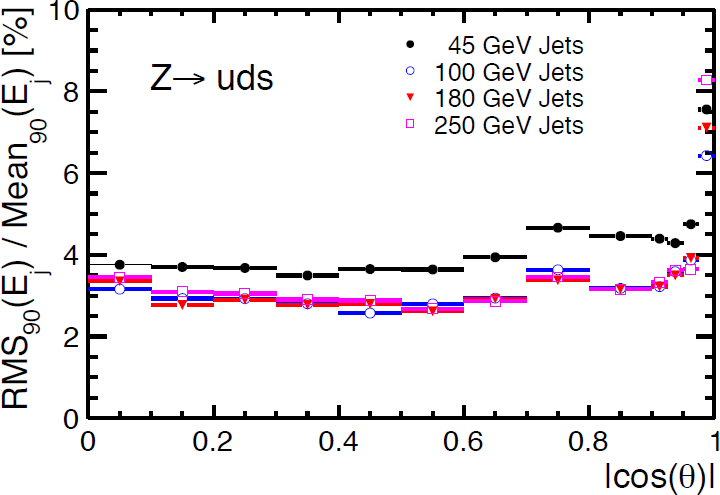
\includegraphics[width=.8\textwidth]{ILD/figs/ResVsCosTheta_ahcal.png}
  \caption{Résolution en énergie des jets en fonction de $|cos\theta|$, dans l'ILD avec le calorimètre hadronique analogique \cite{detectorTDR}.}
  \label{fig:resvscostheta_ahcal}
\end{figure}
La résolution en énergie pour des événements di-jets a déjà été étudiée dans l'ILD avec le calorimètre hadronique à lecture analogique (option avec des scintillateurs de $3\times3~cm^2$) \cite{detectorTDR}. Le calorimètre électromagnétique, utilisé dans cette étude, est le calorimètre SiECAL, avec des galettes de silicium comme milieu actif. Les di-jets sont, ici, issus des désintégrations de bosons Z virtuels en paire de quark-antiquark, lui même généré avec une énergie dans le centre de masse de 91, 200, 360 et 500 $GeV$. Uniquement les quarks légers ($u$, $d$ et $s$) sont considérés dans cette étude. Les quarks sont émis avec la même énergie et une impulsion opposée. Les particules dans les calorimètres sont reconstruites avec un algorithme de suivi des particules que nous présenterons dans la section suivante. La figure~\ref{fig:resvscostheta_ahcal} montre la résolution en énergie des jets ($RMS_{90}/Mean_{90}$) en fonction de $|cos\theta|$, défini par:
\begin{equation}
  |cos\theta| = \frac{1}{\sqrt s}\sum_q{\frac{|p_{z,q}|}{\|\vec p_{q}\|}}
\end{equation}
où $\vec p_{q}$ est l'impulsion du quark $q$ et $p_{z,q}$ sa coordonnée selon l'axe du faisceau.

Comme le montre le tableau~\ref{tab.jetResultAHCAL}, la résolution en énergie des jets est inférieure à 4 $\%$ dans la zone du tonneau du détecteur ($|cos\theta|<0.7$). Les grandeurs $RMS_{90}$ et $Mean_{90}$ correspondent respectivement à l'écart type et la valeur moyenne de la plus petite gamme d'énergie reconstruite contenant 90$\%$ de la statistique. Cette définition de la résolution présente l'avantage d'être relativement peu influencée par les queues de distribution \cite{pfaPandora}. Cependant, le $RMS_{90}$, calculé avec une distribution gaussienne, est plus faible de 21$\%$ que le véritable écart type. Il a ainsi été montré, que la résolution en énergie calculée avec le $RMS_{90}$ devait être multipliée par un facteur 1.1 pour retrouver son équivalent gaussien \cite{pfaPandora}.
\begin{table}[!ht]
  \begin{center}
    \begin{tabular}{r|l}
      \rowcolor{black!20!white} Energie & $\sigma_{E_j}/E_j$ \\
      \hline
      \rowcolor{black!5!white} $45 ~GeV$ & $(3.66\pm0.05)\%$\\
      \rowcolor{black!5!white} $100~GeV$ &$(2.83\pm0.04)\%$\\
      \rowcolor{black!5!white} $180~GeV$ &$(2.86\pm0.04)\%$\\
      \rowcolor{black!5!white} $250~GeV$ &$(2.95\pm0.04)\%$\\
    \end{tabular}
  \end{center}  
  \caption{Résolution en énergie des jets dans la région du tonneau ($|cos\theta|<0.7$). La résolution en énergie des jets est calculée à partir du $RMS_{90}$ \cite{detectorTDR}.}
  \label{tab.jetResultAHCAL}
\end{table}

\begin{figure}[!ht]
  \subfigure[]{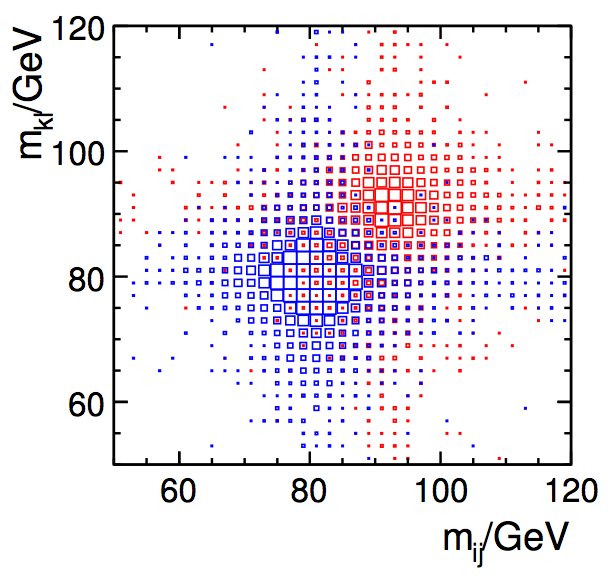
\includegraphics[width=.49\textwidth]{ILD/figs/DijetMass.png}}
  \subfigure[]{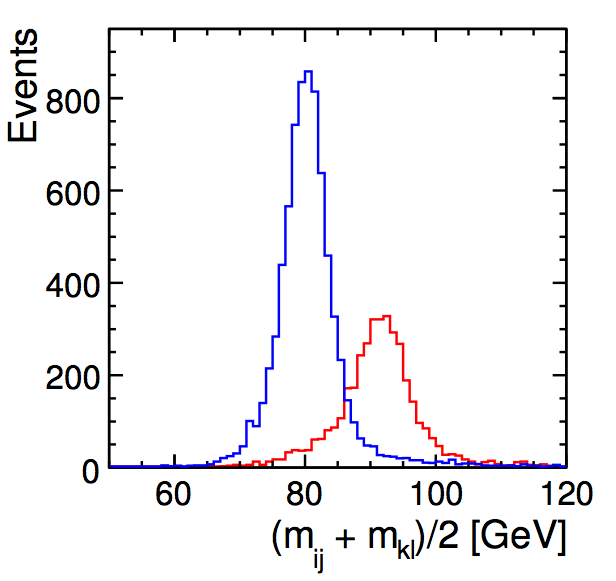
\includegraphics[width=.49\textwidth]{ILD/figs/WZseparation.png}}
  \caption{(a): Masse des di-jets reconstruits pour des simulations d'événements $e^+e^-\rightarrow\nu_e\bar{\nu_e}W^+W^-$ (en bleu) et $e^+e^-\rightarrow\nu_e\bar{\nu_e}ZZ$ (en rouge) à $\sqrt{s}=1~TeV$. (b): Distribution de la masse moyenne des di-jets reconstruits $(m_{ij}+m_{ik})/2$ pour les événements $e^+e^-\rightarrow\nu_e\bar{\nu_e}W^+W^-$ (en bleu) et $e^+e^-\rightarrow\nu_e\bar{\nu_e}ZZ$ (en rouge) \cite{detectorTDR}.}
  \label{fig:ww-zz-ahcal}
\end{figure}
La reconstruction de la masse des bosons W et Z a aussi été étudiée dans l'ILD avec le calorimètre hadronique analogique, en utilisant les technique de suivi des particules. Cette étude est basée sur l'analyse des réactions $e^+e^-\rightarrow\nu_e\bar{\nu_e}W^+W^-$ et $e^+e^-\rightarrow\nu_e\bar{\nu_e}ZZ$, où les bosons W et Z se désintègrent en paire de quarks ou d'antiquarks ou en paire de quark-antiquark. La figure~\ref{fig:ww-zz-ahcal}(a) montre les masses des di-jets reconstruits pour les meilleures associations de jets\footnote{Les meilleures associations de paires de jets sont obtenues en minimisant $|m_{ij}-m_{W/Z}|\times|m_{kl}-m_{W/Z}|$.} pour des événements $e^+e^-\rightarrow\nu_e\bar{\nu_e}W^+W^-$ et $e^+e^-\rightarrow\nu_e\bar{\nu_e}ZZ$ à $\sqrt{s}=1~TeV$. La figure~\ref{fig:ww-zz-ahcal}(b) montre la distribution de la moyenne des deux masses des di-jets reconstruits. Ces deux figures indiquent une séparation claire de la masse des bosons de jauge et valident le concept de suivi des particules.

\newpage
\section{Identification et séparation des dépôts électromagnétiques et hadroniques dans l'ILD}
\label{sec.pandora}
La reconstruction des particules est réalisée à l'aide de l'algorithme PandoraPFA \cite{pfaPandora}. Le but de cet algorithme est de combiner les informations relatives aux traces, laissées par les particules chargées dans le trajectographe, avec les hits dans les calorimètres ultra-granulaires. Ces combinaisons doivent permettre de reconstruire toutes les particules individuelles dans les jets. Les principales étapes de l'algorithme sont les suivantes \cite{pfaPandora}:
\begin{enumerate}[~~1-]
\item Les traces dont la topologie est remarquable comme celles issues de la désintégration de particules neutres dans le trajectographe (exemple: $K_s\rightarrow \pi^+\pi^-$) sont identifiées.
\item Des amas dans les calorimètres sont créés en agglomérant les hits dans des cônes, en allant des couches internes vers les plus externes. La projection des traces dans les calorimètres est utilisée comme graine pour démarrer cette procédure. Des amas sont alors associés aux traces dans le trajectographe. Les autres sont considérés comme neutres.
\item Les amas neutres peuvent être ajoutés dans ceux déjà associés à une trace, lorsqu'ils sont topologiquement compatibles;
\item L'énergie des amas associés est alors comparée à celle des traces. Dans les cas où l'énergie d'un amas ne correspond pas à l'énergie d'une trace, la procédure de création des amas est relancée en modifiant les paramètres géométriques des cônes, avec l'espoir d'obtenir une meilleure correspondance. 
\item La dernière étape consiste à créer les objets informatiques correspondant aux particules reconstruites. L'énergie des particules chargées est alors calculée avec les impulsions des traces mesurées dans le trajectographe. L'énergie des particules neutres est mesurée avec l'information des hits dans les calorimètres.
\end{enumerate}
Notons enfin, que cet algorithme a été optimisé pour améliorer les performances de l'ILD avec le calorimètre hadronique analogique.

\section{Reconstruction de l'énergie des jets avec le SDHCAL}
\subsection{Simulation du SDHCAL dans l'ILD}
\label{sec.ildSDHCALSIM}
La simulation du SDHCAL et particulièrement la modélisation de la réponse des GRPC sont ici légèrement différentes de celles présentées dans le chapitre~\ref{chap.simulation}. Premièrement, la procédure, visant à relier les segments GEANT4 lorsqu'ils appartiennent à la même particule dans la même couche de gaz, n'est pas effectuée. De plus, pour des raisons de format de données, il n'était pas possible de conserver les informations relatives aux positions d'entrée et de sortie, dans la couche de gaz, des segments GEANT4. La correction de la charge induite en fonction de la longueur du segment ($Q_{corr}=Q_{ind}(\frac{d_s}{d_{gap}})^\kappa$ dans la section~\ref{sec.algo} du chapitre~\ref{chap.simulation}) n'est donc pas appliquée. Les paramètres de l'algorithme SimDigital (ceux de la distribution de Polya, ceux responsables de la répartition de la charge et celui modélisant l'écrantage de la charge) ont tout de même été optimisés pour reproduire:
\begin{enumerate}[-]
\item le spectre de charge obtenu avec le scan en seuil;
\item la multiplicité (nombre de cellules touchées lorsqu'une seule particule traverse la couche de gaz) mesurée avec les événements muons, parallèles à l'axe du faisceau, dans le prototype;
\item le nombre total de hits dans les gerbes électromagnétiques.
\end{enumerate}

Enfin, la version actuelle de l'algorithme de reconstruction des particules utilisé (cf. section~\ref{sec.pandora}), impose de fournir une formule de reconstruction de l'énergie linéaire. Nous avons choisi une formule de la forme
\begin{equation}
E_{reco}=\alpha N1 + \beta N2 + \gamma N3
\end{equation}
où $N1$, $N2$ et $N3$ correspondent aux nombres de hits relatifs à chaque seuil et $\alpha$, $\beta$ et $\gamma$ sont des constantes. Nous avons montré, dans le chapitre~\ref{chap.sdhcal} section~\ref{sec.ereco}, qu'une formule, utilisant des fonctions quadratiques du nombre total de hits à la place des coefficents constants, est plus adaptée.
\begin{figure}[!ht]
  \subfigure[]{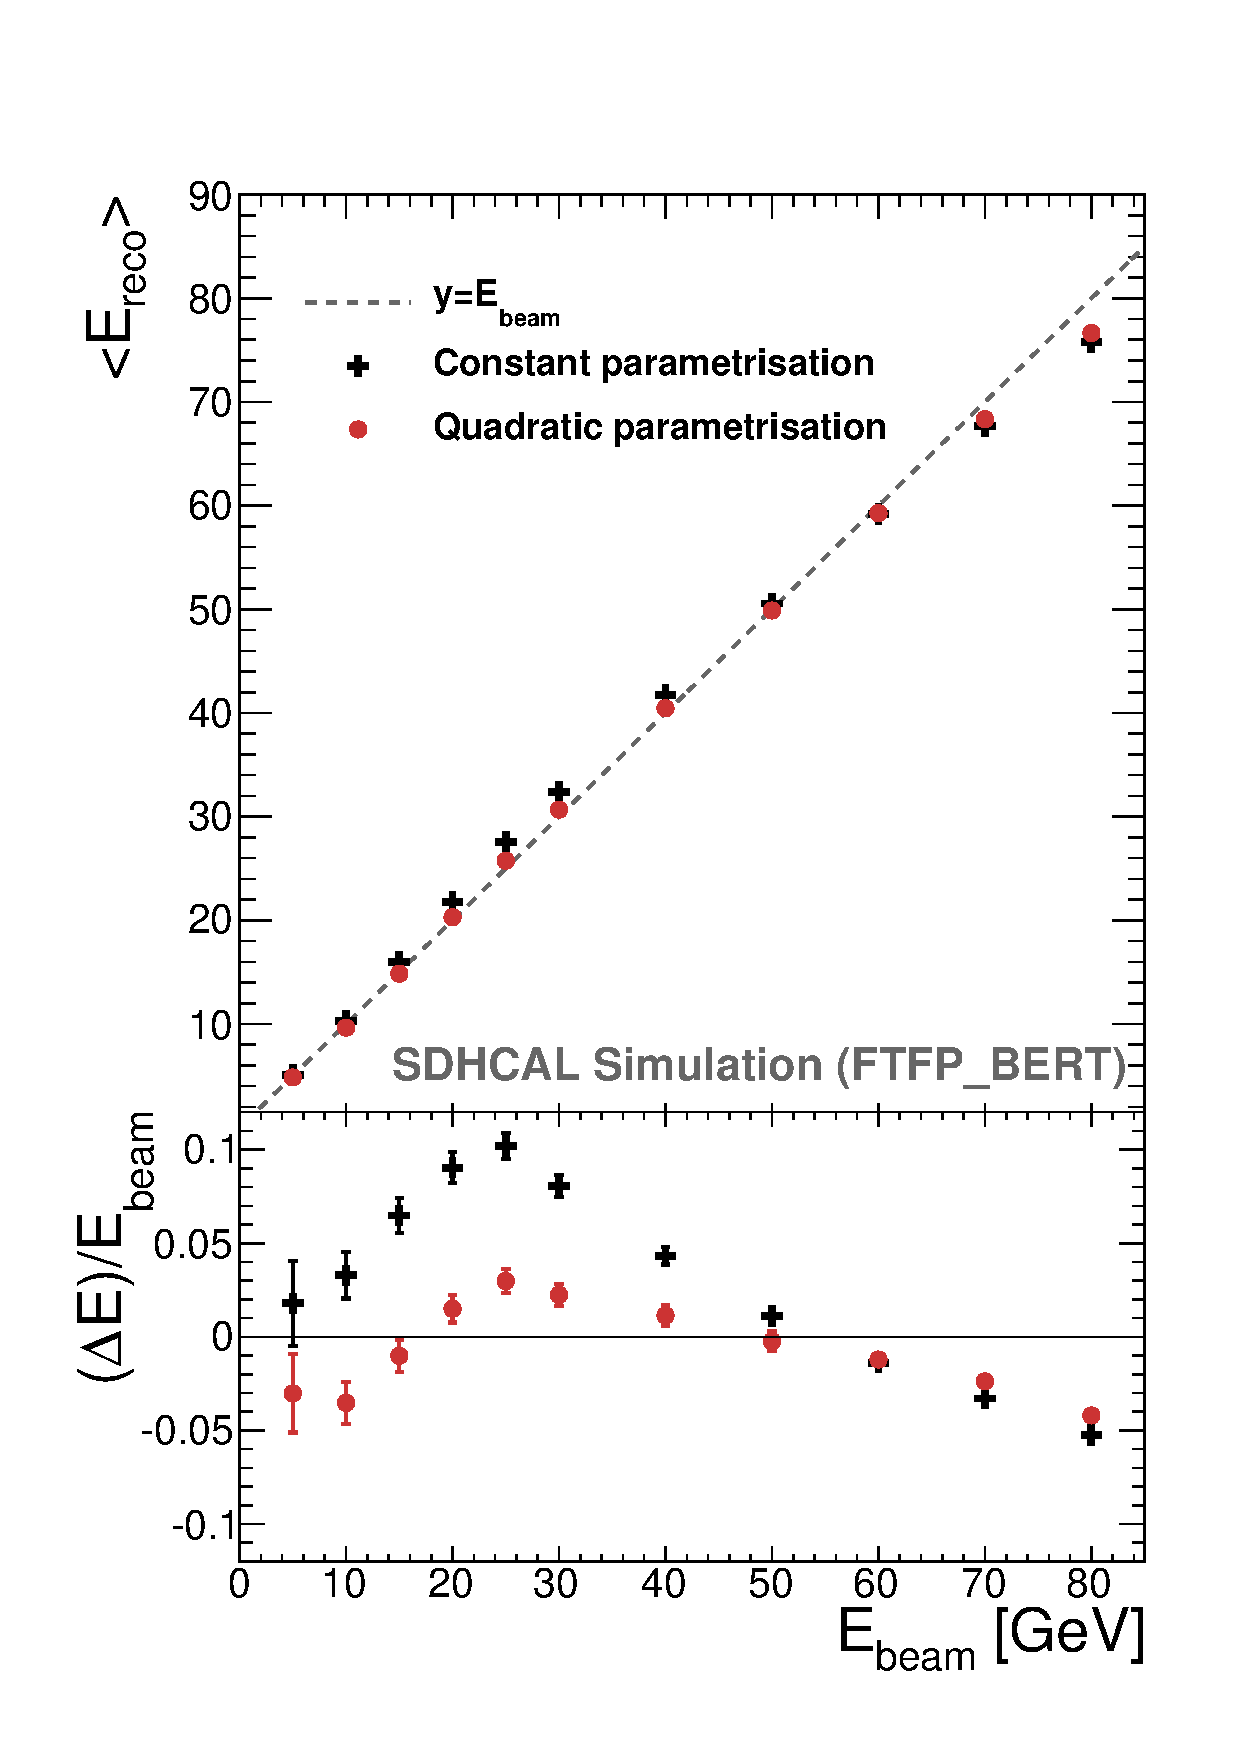
\includegraphics[width=.45\textwidth]{ILD/figs/EREC.pdf}}
  \subfigure[]{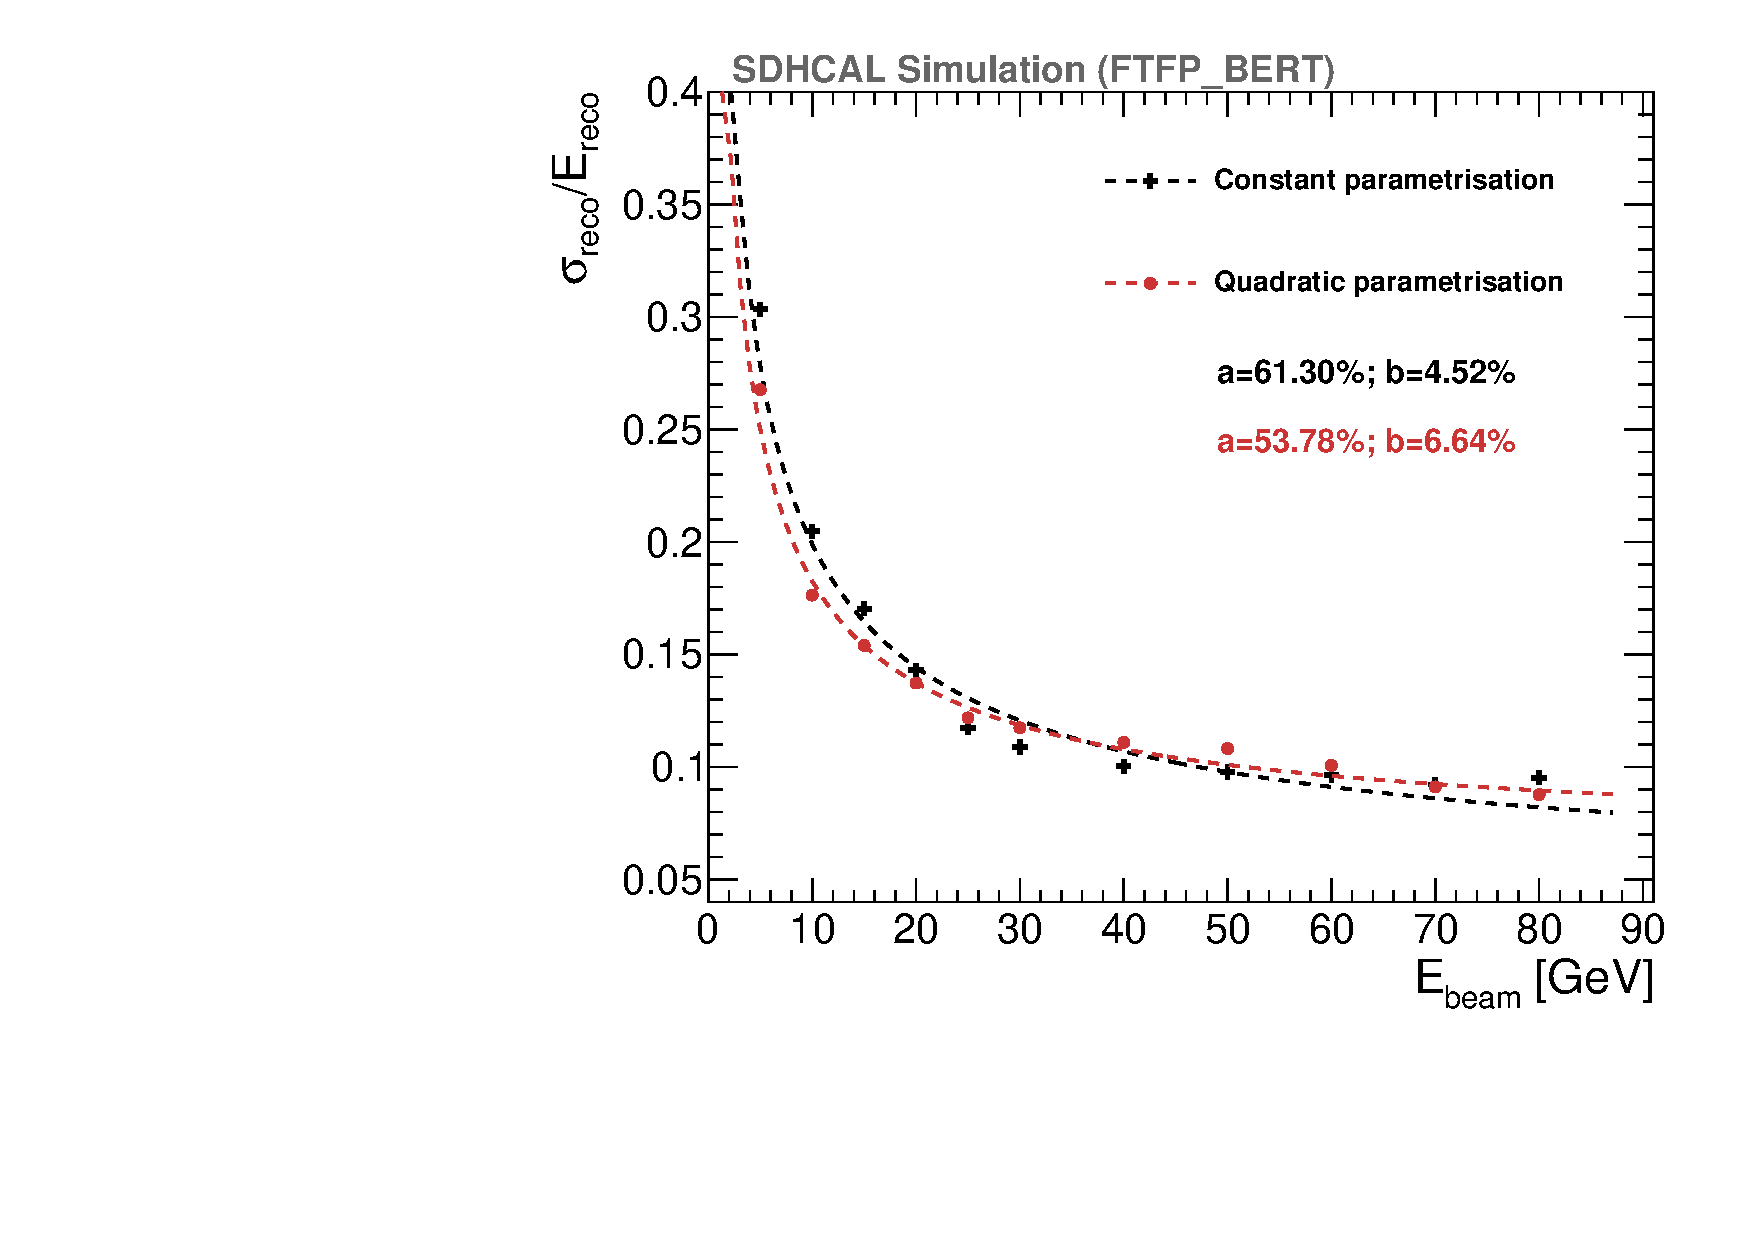
\includegraphics[width=.55\textwidth]{ILD/figs/ERES.pdf}}
  \caption{Énergie reconstruite moyenne (a) et résolution en énergie (b) en fonction de l'énergie de la particule incidente, en utilisant la formule à coefficients constants (ligne noire) et en utilisant le paramétrage quadratique (en rouge).}
  \label{fig:sdhcal-erec-eres}
\end{figure}
Pour chacune des deux méthodes, la procédure de reconstruction de l'énergie de gerbes hadroniques a été réalisée avec des échantillons de simulation, utilisant la liste physique FTFP\_BERT, de 5 à 80 $GeV$. La figure~\ref{fig:sdhcal-erec-eres}(a) présente les valeurs moyennes d'énergie reconstruite en fonction de l'énergie du pion incident. Entre 10 à 50 $GeV$, la méthode, utilisant des coefficients constants, surestime significativement l'énergie de la particule incidente. La figure~\ref{fig:sdhcal-erec-eres}(b) présente la résolution en énergie $\sigma_{reco}/E_{reco}$ en fonction de l'énergie pour les deux méthodes. A basse énergie, l'utilisation du paramétrage quadratique des coefficients améliore sensiblement la résolution. Ces deux courbes sont ajustées avec la fonction:
\begin{equation}
  \frac{\sigma_{reco}}{E_{reco}}=\frac{a}{\sqrt{E_{beam}}} \oplus b
\end{equation}
où $E_{beam}$ est l'énergie du pion incident. La méthode utilisant le paramétrage quadratique permet d'obtenir un meilleur terme stochastique $a$ mais le terme constant $b$ est plus élevé. Cependant, la transposition du paramétrage quadratique dans l'ILD n'est pas triviale car les dépôts énergétiques se trouvent à la fois dans le calorimètre électromagnétique et dans le calorimètre hadronique. Ce développement sera un des axes de travail pour améliorer les performances de reconstruction des jets avec le SDHCAL.

\subsection{Energie reconstruite des jets}
\begin{figure}[!ht]
  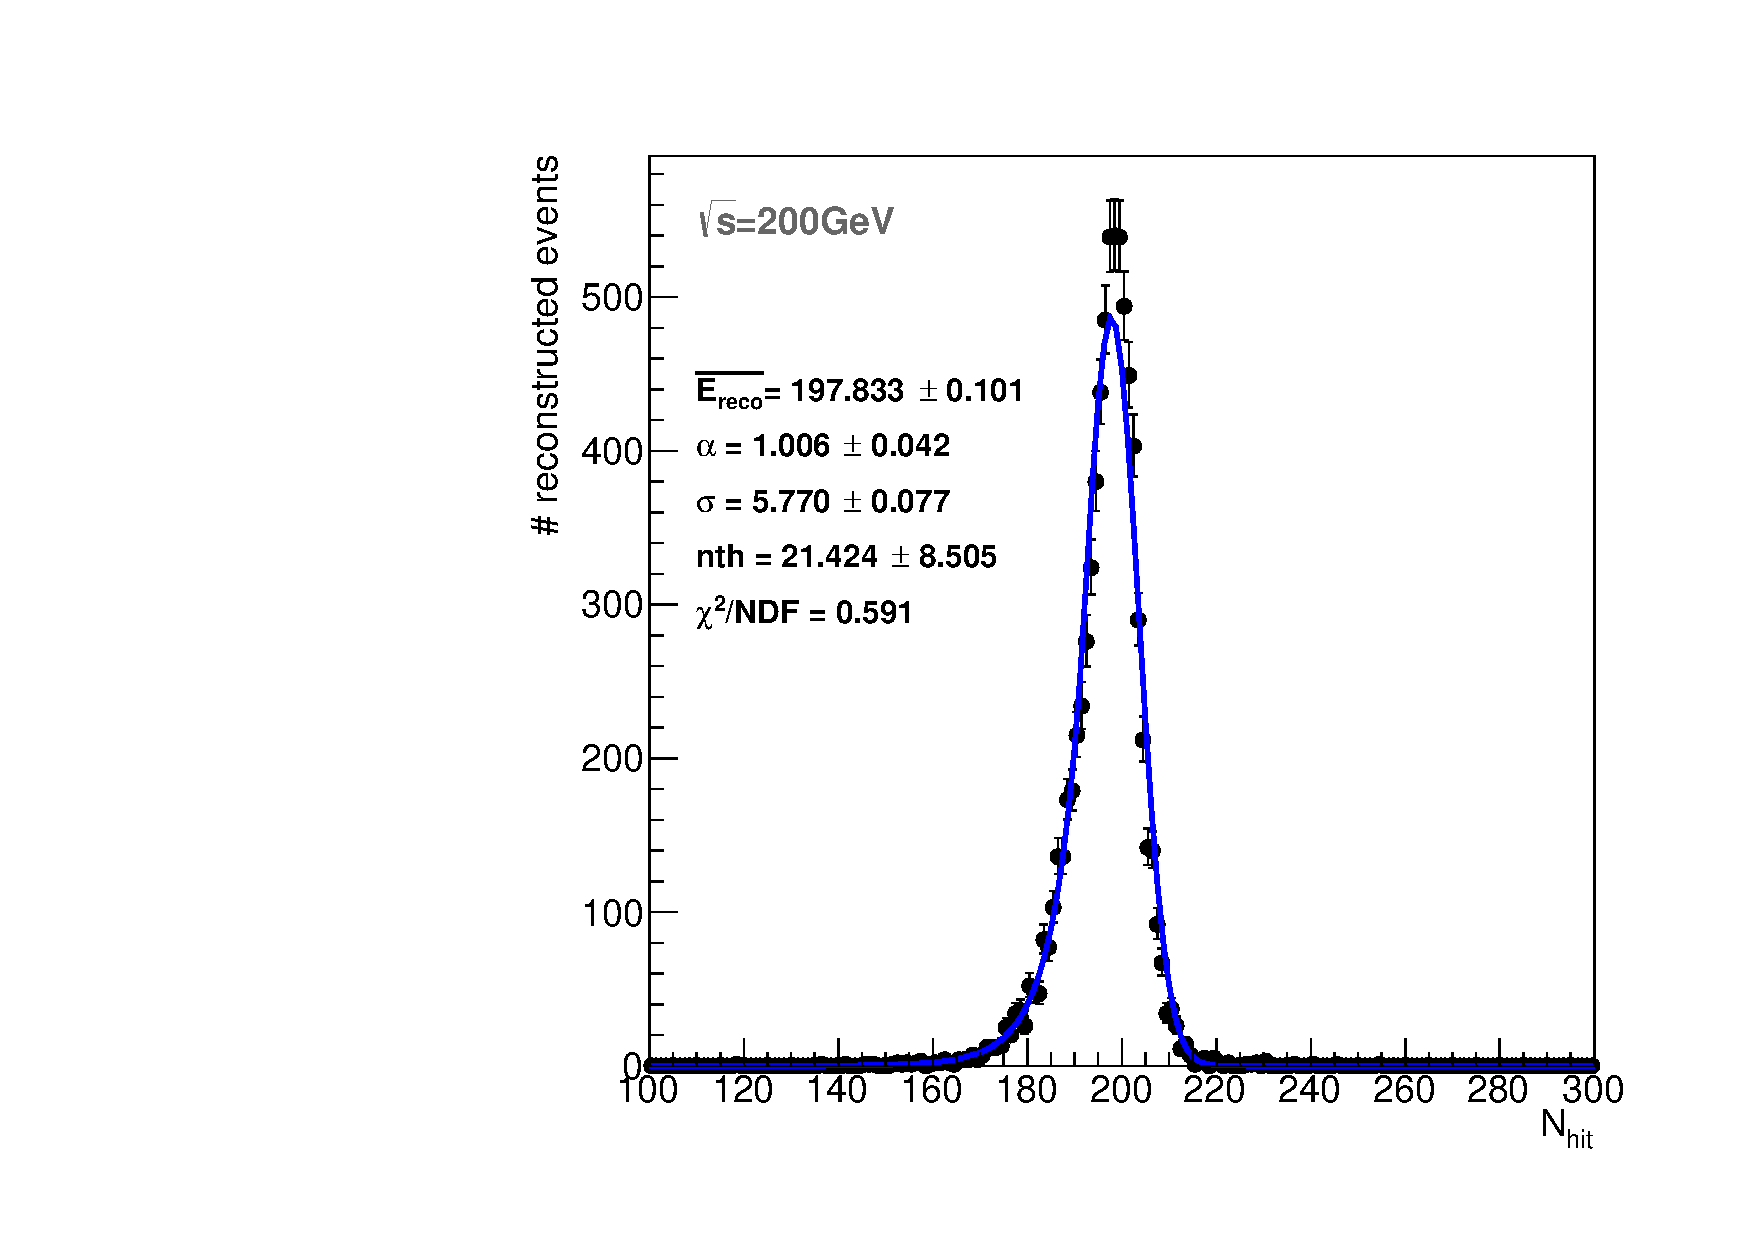
\includegraphics[width=.49\textwidth]{ILD/figs/erec_200GeV_fPFA.pdf}
  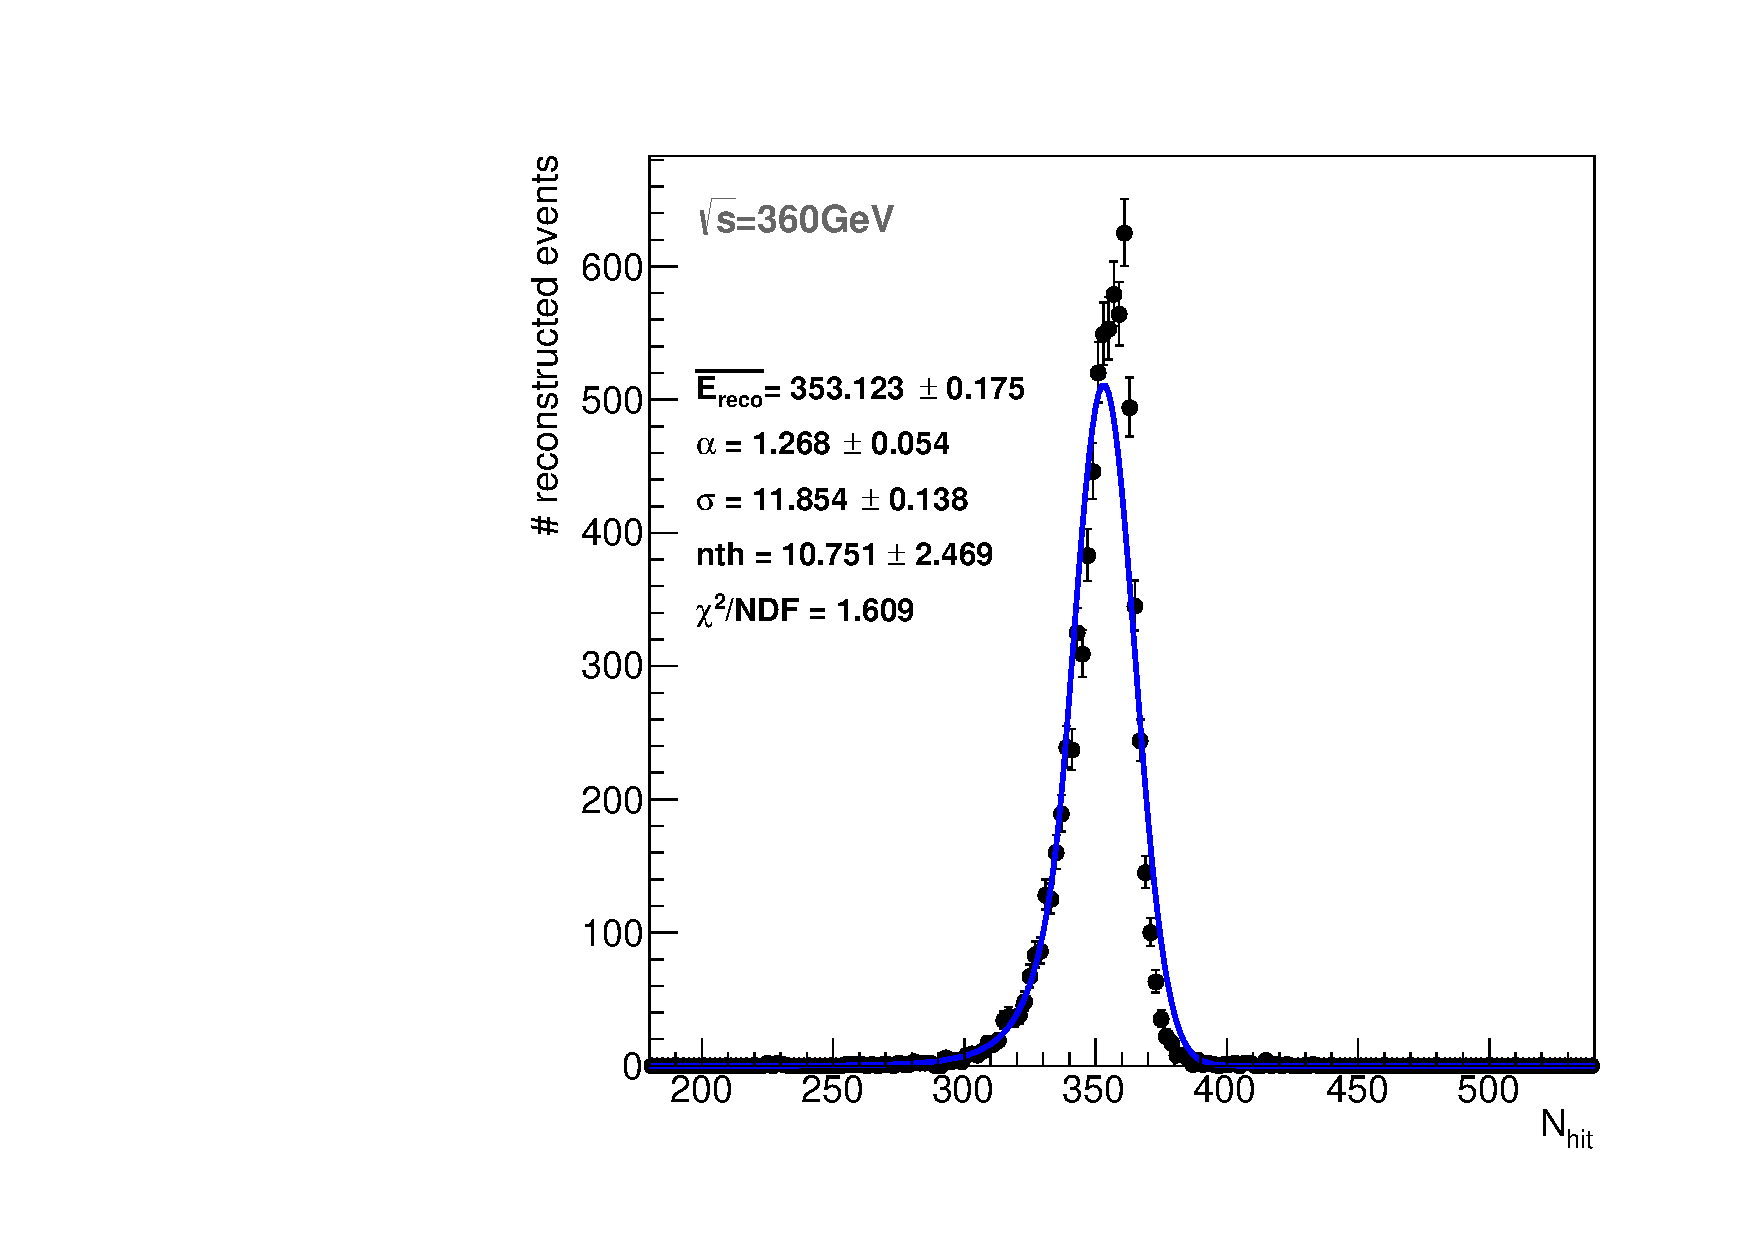
\includegraphics[width=.49\textwidth]{ILD/figs/erec_360GeV_fPFA.pdf}
  \caption{Energie totale reconstruite pour des événéments $e^+e^-\rightarrow Z \rightarrow q\bar{q}$ à $\sqrt{s}=$ 200 (à gauche) et 360 (à droite) $GeV$.}
  \label{fig:jet-energy}
\end{figure}
Les mêmes événements di-jets, utilisés dans la section~\ref{sec.jetintro}, sont considérés pour étudier les performances de l'ILD avec le calorimètre électromagnétique SiECAL et le calorimètre hadronique à lecture semi-digitale. La simulation du détecteur complet est réalisée avec le logiciel Mokka \cite{mokka}. Ce logiciel utilise GEANT4 et une description réaliste de la géométrie du détecteur et de ses sous-détecteurs. La reconstruction des particules utilise l'algorithme PandoraPFA (cf. section~\ref{sec.pandora}). La figure ~\ref{fig:jet-energy} présente la distribution en énergie reconstruite des di-jets pour des énergies dans le centre de masse de 200 et 360 $GeV$. L'énergie moyenne et la résolution des distributions en énergie reconstruites sont détererminées par la méthode du $RMS_{90}$. La résolution en énergie $\sigma_j/E_j$ des jets est finalement donnée par:
\begin{equation}
\frac{\sigma_j}{E_j}=\frac{RMS_{90}/\sqrt{2}}{Mean_{90}/2}=\sqrt{2}\frac{RMS_{90}}{Mean_{90}}
\end{equation}

\begin{figure}[!ht]
  \centering
  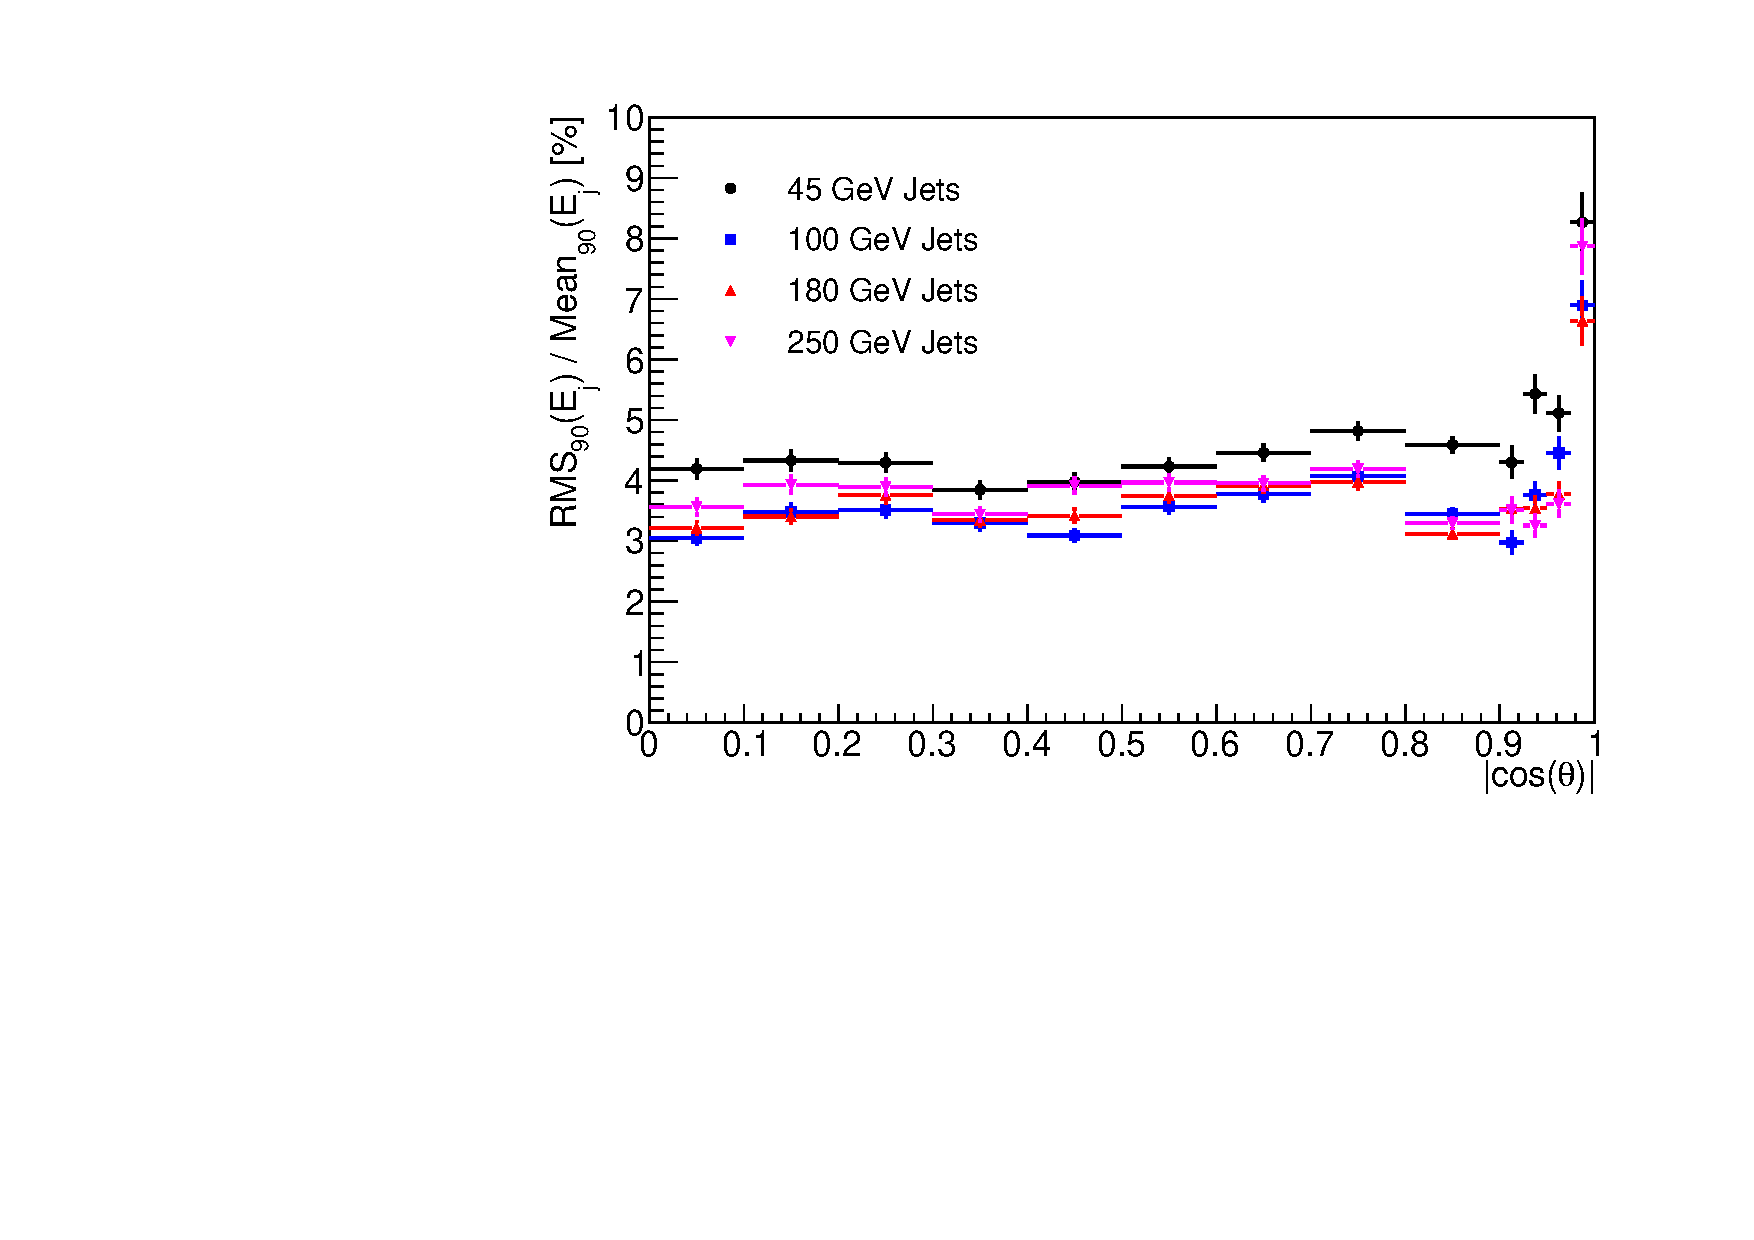
\includegraphics[width=.8\textwidth]{ILD/figs/ResVsCosTheta.pdf}
  \caption{Résolution en énergie des jets en fonction de $|cos\theta|$ pour des jets de 45, 100, 180 et 250 $GeV$, avec le SDHCAL.}
  \label{fig:jet-energy-vs-costheta}
\end{figure}
La figure~\ref{fig:jet-energy-vs-costheta} présente la résolution en énergie des jets en fonction de $|cos\theta|$. 
\begin{table}[!ht]
  \begin{center}
    \begin{tabular}{r|l}
      \rowcolor{black!20!white} Energie & $\sigma_{E_j}/E_j$ \\
      \hline
      \rowcolor{black!5!white} $45 ~GeV$ & $(4.19\pm0.06)\%$\\
      \rowcolor{black!5!white} $100~GeV$ &$(3.36\pm0.05)\%$\\
      \rowcolor{black!5!white} $180~GeV$ &$(3.52\pm0.05)\%$\\
      \rowcolor{black!5!white} $250~GeV$ &$(3.79\pm0.06)\%$\\
    \end{tabular}
  \end{center}  
  \caption{Résolution en énergie des jets dans la région du tonneau ($|cos\theta|<0.7$) avec le SDHCAL. La résolution en énergie des jets est calculée à partir du $RMS_{90}$.}
  \label{tab.jetResultSDHCAL}
\end{table}
Le tableau~\ref{tab.jetResultSDHCAL} présente la résolution en énergie des jets dans la région du tonneau avec le SDHCAL. Ces résultats respectent les performances de référence pour la reconstruction de jets dans l'ILC. Cependant, les résolutions en énergie des jets obtenues avec le calorimètre hadronique semi-digital sont légèrement moins bonnes que celles obtenues avec le calorimètre analogique. Plusieurs pistes de travail pourraient permettre d'améliorer ces résultats. Nous avons vu dans la section~\ref{sec.ildSDHCALSIM} que la reconstruction de l'énergie des gerbes hadroniques est plus efficace en utilisant un paramétrage quadratique. De plus, l'algorithme de reconstruction PandoraPFA (cf. section~\ref{sec.pandora}) a fortement été optimisé avec le calorimètre analogique. Une collaboration, avec les développeurs de cet algorithme, a récemment été débutée pour essayer de mieux l'adapter au SDHCAL. Enfin, un algorithme, basé sur une autre technique de reconstruction essayant de tirer un maximum de profit de la granularité du SDHCAL, est en cours de développement au sein de l'Institut de Physique Nucléaire de Lyon.

\section{Reconstruction des événements WW et ZZ}
La reconstruction des masses des bosons W et Z est réalisée pour les réactions $e^+e^-\rightarrow W^+W^-$ et $e^+e^-\rightarrow ZZ$. 
\begin{figure}[!ht]
  \centering
  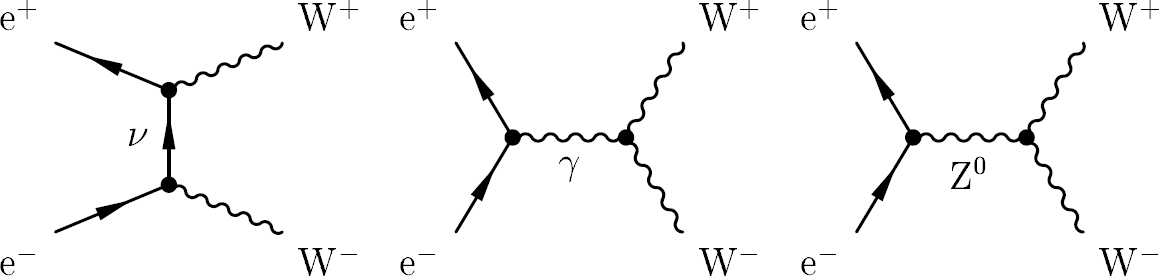
\includegraphics[width=.8\textwidth]{ILD/figs/wwFeynman.png}
  \caption{Principaux diagrammes de production de paires $W^+W^-$ à l'ILC \cite{physicsTDR}.}
  \label{fig:wwFeynman}
\end{figure}
La figure~\ref{fig:wwFeynman} présente les principaux diagrammes de Feynman pour la production de paires $W^+W^-$ à l'ILC. Uniquement les désintégrations hadroniques des bosons de jauges sont considérée s dans cette étude. Les réactions sont simulées à l'aide du générateur Whizard \cite{whizard}. La simulation de l'interaction des particules issues du générateur avec les sous-détecteurs est de nouveau réalisée avec Mokka et la reconstruction des particules avec l'algorithme PandoraPFA. Ces particules reconstruites doivent ensuite être regroupées dans des jets. Nous avons utilisé l'algorithme $k_t$ disponible dans la librairie FastJet \cite{fastJet}. Le nombre de jets à reconstruire est fixé à quatre. Les jets sont ensuite combinés en di-jets pour reconstruire les bosons de jauge W et Z. La meilleure combinaison de di-jets est obtenue en minimisant le $\chi^2$ suivant:
\begin{equation}
  \chi^2= \big( \sqrt{s}-E_1-E_2 \big)^2 + \|\vec{p_{1}}+\vec{p_2}\|^2 + \big(M_1-M_2\big)^2
\end{equation}
où $E_i$, $\vec{p_i}$ et $M_i$ correspondent à l'énergie du di-jet $i$, son impulsion et sa masse. 

\begin{figure}[!ht]
  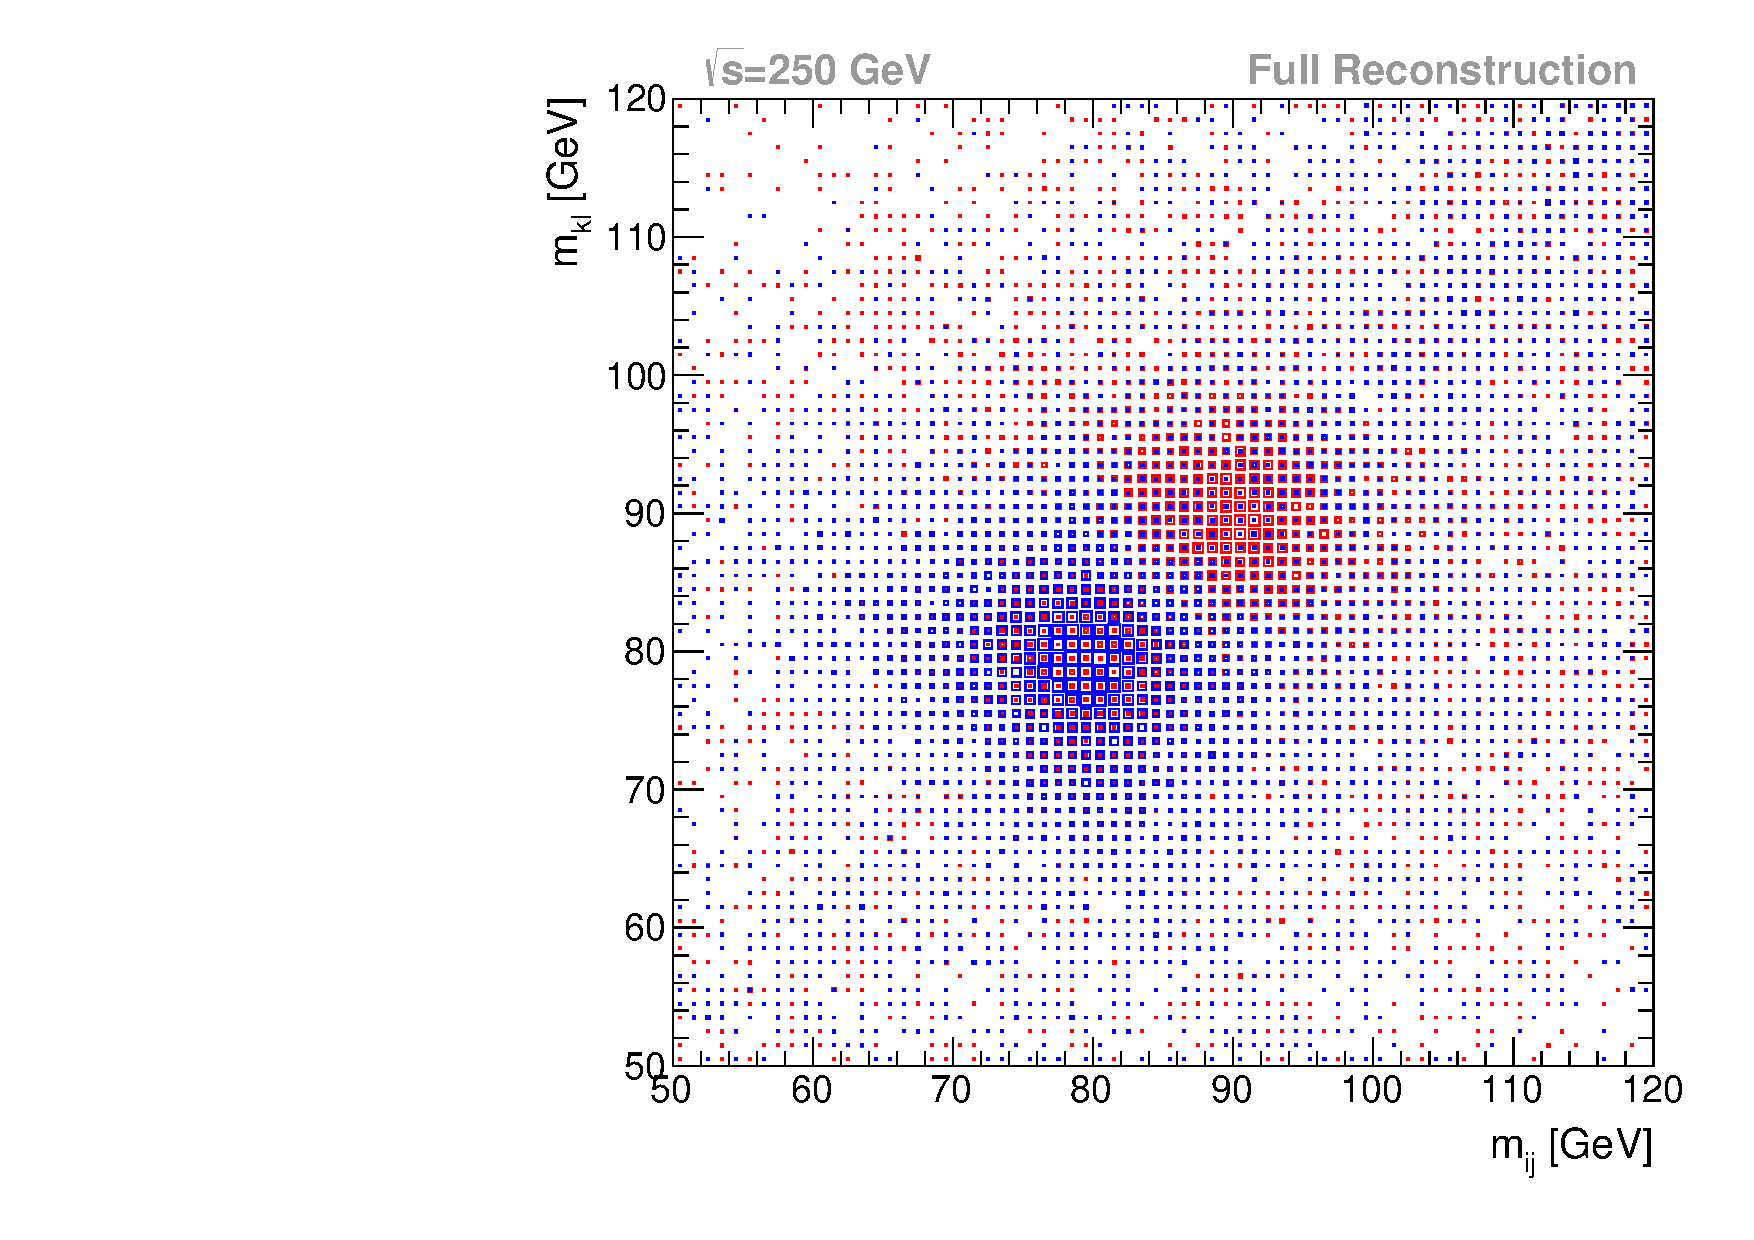
\includegraphics[width=.49\textwidth]{ILD/figs/mIJ_vs_mKL.pdf}
  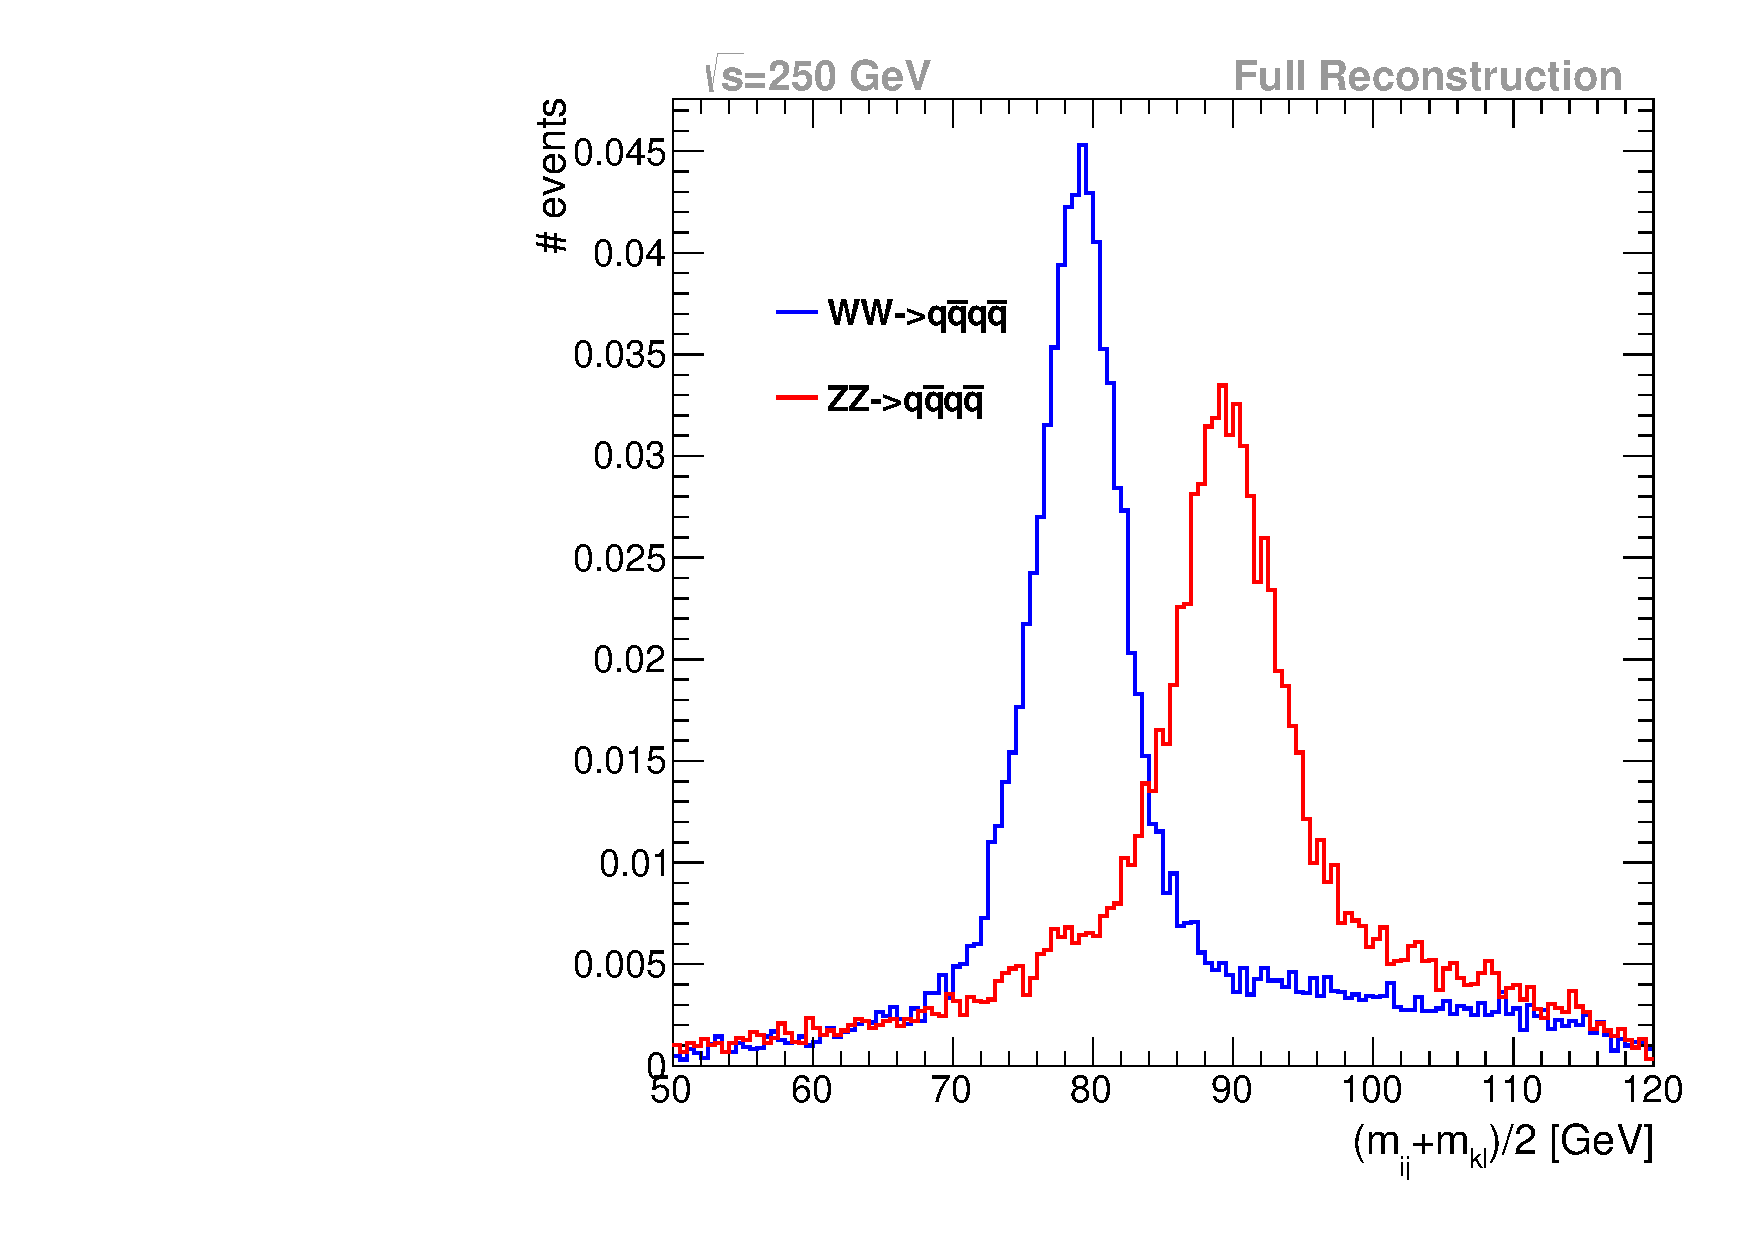
\includegraphics[width=.49\textwidth]{ILD/figs/mass_distrib.pdf}
  \caption{(a): Masse des di-jets reconstruits pour des simulations d'événements $e^+e^-\rightarrow W^+W^-$ (en bleu) et $e^+e^-\rightarrow ZZ$ (en rouge) à $\sqrt{s}=250~GeV$. (b): Distribution de la masse moyenne des di-jets reconstruits $(m_{ij}+m_{ik})/2$. Ces distributions sont normalisées aux nombres d'événements. Les événements sont reconstruits dans une simulation complète de l'ILD avec le SDHCAL.}
  \label{fig:ww-zz-mass}
\end{figure}
La figure~\ref{fig:ww-zz-mass}(a) montre les masses des di-jets reconstruits pour des événements $e^+e^-\rightarrow W^+W^-$ et $e^+e^-\rightarrow ZZ$ à $\sqrt{s}=250~GeV$. La figure~\ref{fig:ww-zz-mass}(b) montre la distribution de la moyenne des deux masses des di-jets reconstruits. Ces deux figures indiquent une séparation raisonnable de la masse des bosons de jauge. Cependant les queues dans les distributions de masse sont importantes. La même procédure de reconstruction des jets a été réalisée avec les particules issues du générateur Whizard. Ces résultats sont présentés par la figure~\ref{fig:ww-zz-mass_MC}.
\begin{figure}[!ht]
  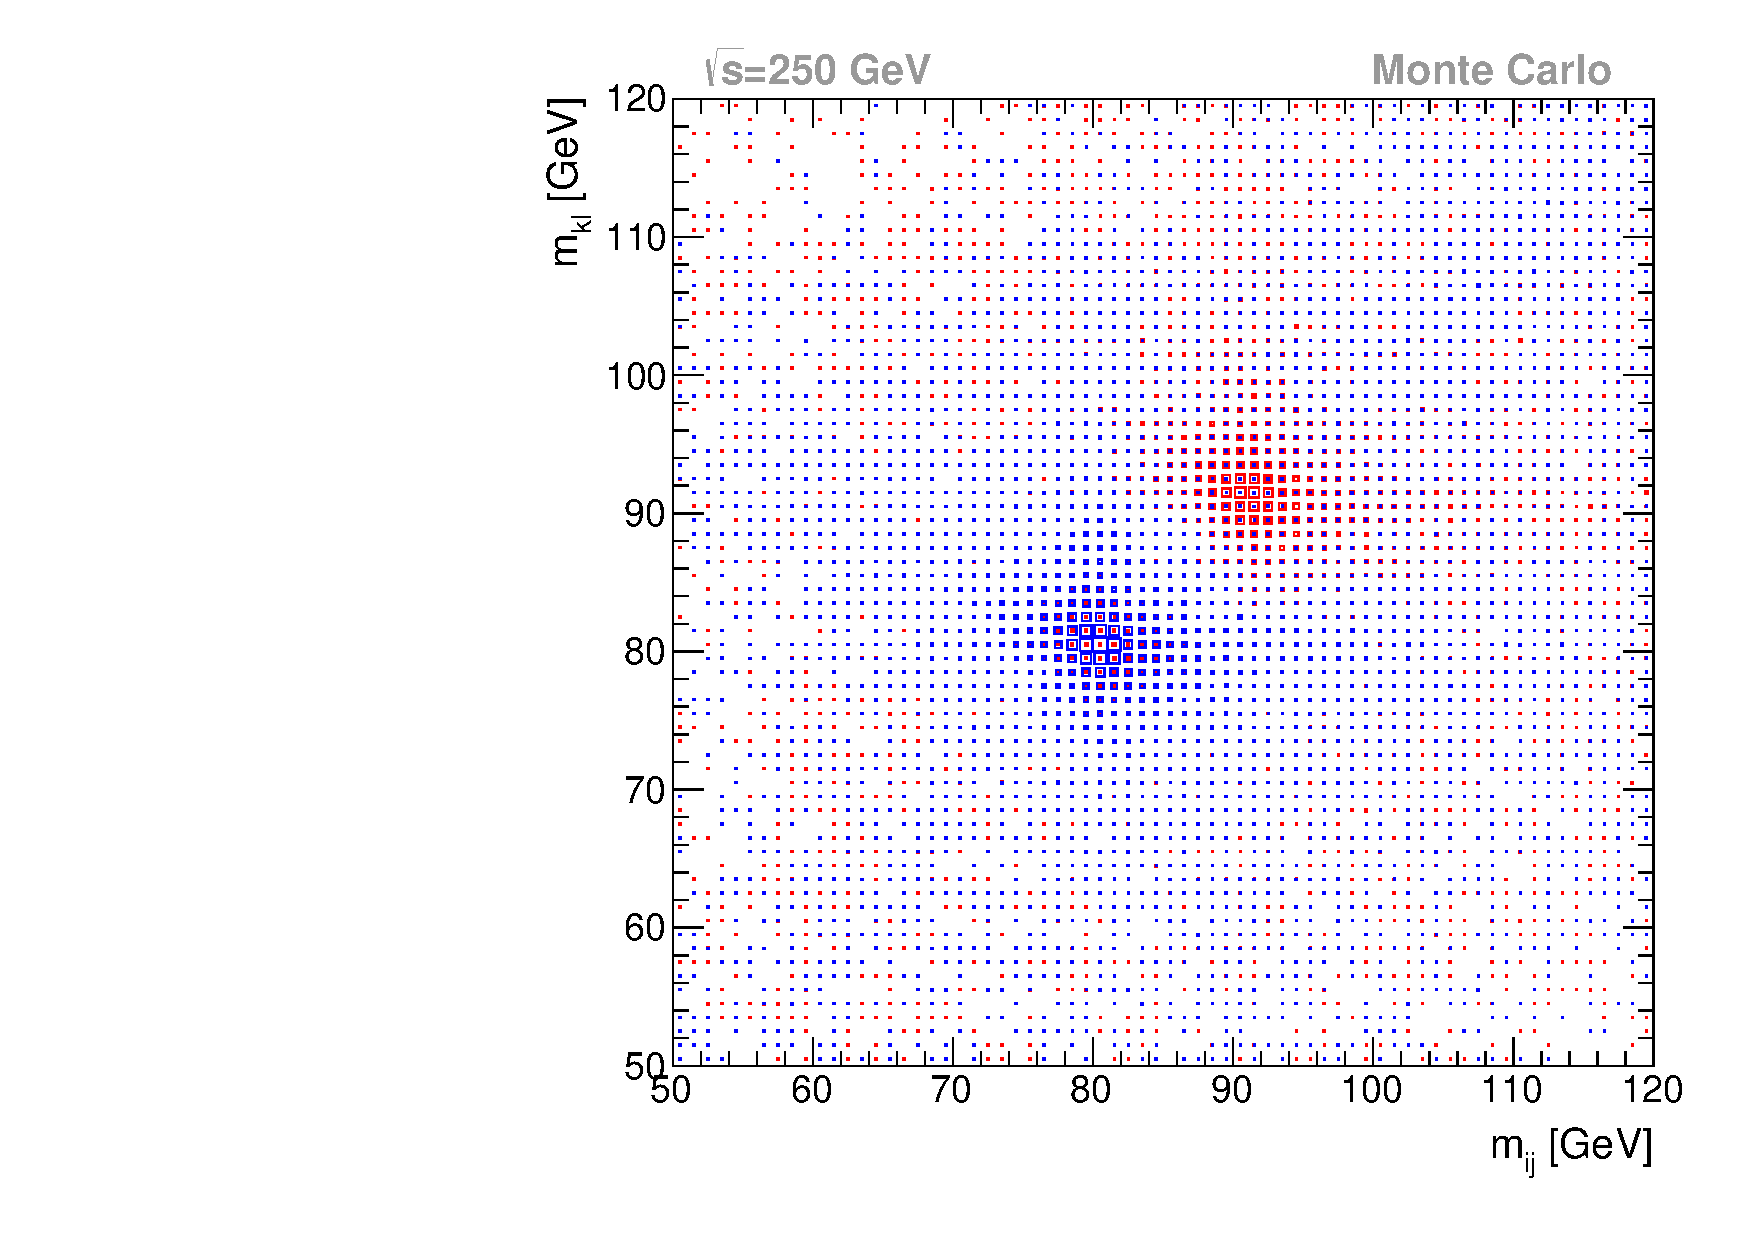
\includegraphics[width=.49\textwidth]{ILD/figs/mIJ_vs_mKL_MC.pdf}
  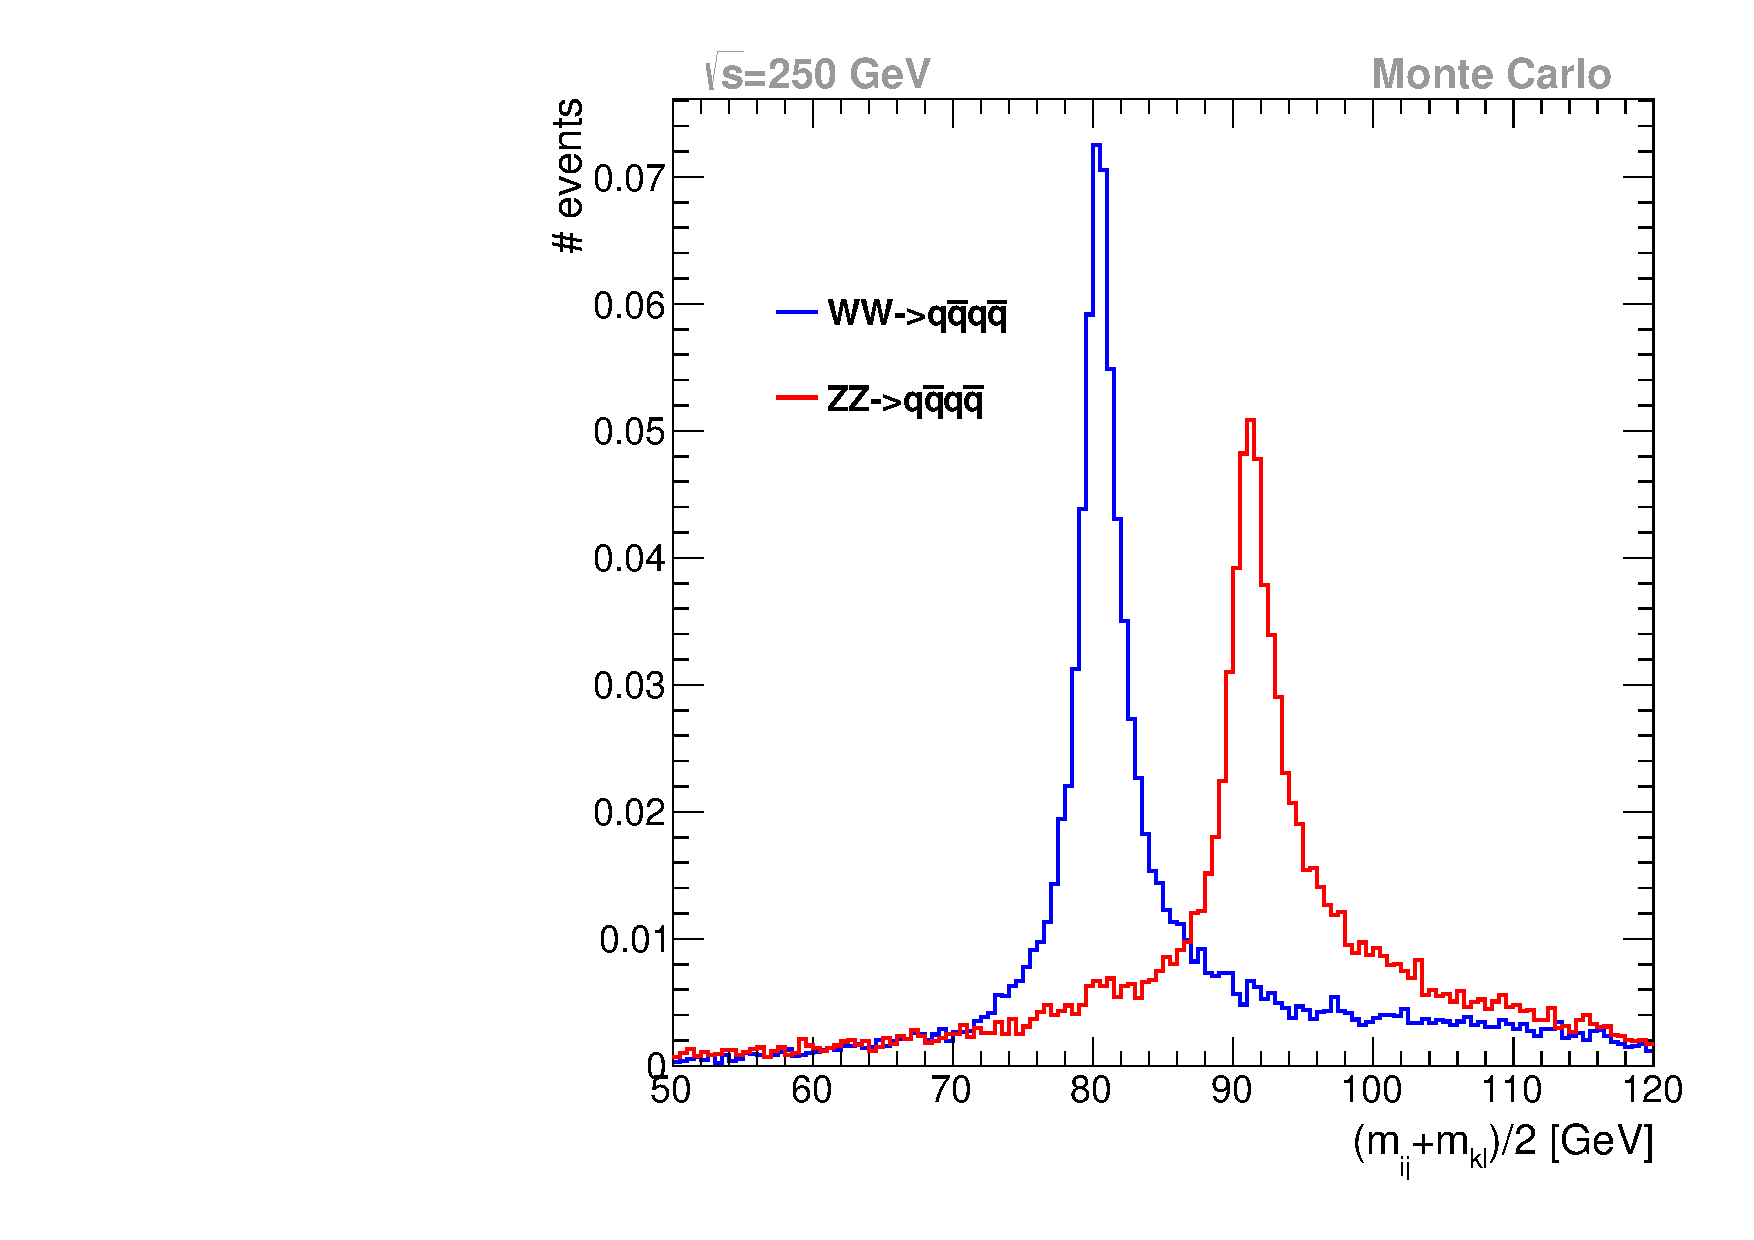
\includegraphics[width=.49\textwidth]{ILD/figs/mass_distrib_MC.pdf}
  \caption{(a): Masse des di-jets reconstruits pour des simulations d'événements $e^+e^-\rightarrow W^+W^-$ (en bleu) et $e^+e^-\rightarrow ZZ$ (en rouge) à $\sqrt{s}=250~GeV$. (b): Distribution de la masse moyenne des di-jets reconstruits $(m_{ij}+m_{ik})/2$. Ces distributions sont normalisées aux nombres d'événements. Les événements sont reconstruits à partir des particules produites dans le générateur Whizard.}
  \label{fig:ww-zz-mass_MC}
\end{figure}
 Les queues des distributions de masse sont aussi présentes, ce qui indique que la construction et/ou l'association des jets utilisées ne sont pas optimales. Aucun traitement adapté aux bruits de fond dû aux photons, n'a effectivement été réalisé. 

\newpage
\section{Conclusion}
Les résultats sur la résolution en énergie des jets et la reconstruction des masses des bosons $W$ et $Z$ obtenus avec la simulation de l'ILD avec le SDHCAL sont encourageants. La résolution en énergie des jets respecte les performances de référence pour la reconstruction de jets dans l'ILC. Ces résultats pourront même être améliorés en utilisant une formule de reconstruction de l'énergie des gerbes hadroniques plus adaptée. De plus, l'algorithme de reconstruction des particules est en cours d'optimisation avec le SDHCAL et un autre algorithme est aussi en phase de développement. Les masses des bosons $Z$ et $W$ sont raisonnablement bien séparées malgré la présence de queues dans les distributions. 
